\setlength{\footskip}{8mm}

\chapter{Data preprocessing \& data-warehouse}
\label{ch:dpdd}
This chapter presents the progress in data preprocessing and data-warehouse development.

\section{Data collection}
The data was collected from the open source data available at SGI MLC++ website hosted at : \url{https://www.sgi.com/tech/mlc/db/}. The site has two files suitable for churn prediction. The data was donated to the public domain by Orange telecom.
\begin{itemize}
	\item Data file \textit{``churn.all``} at location  \textit{\url{https://www.sgi.com/tech/mlc/db/churn.all}}.
	\item Meta-data file \textit{``churn.names``} for the data at location \textit{\url{https://www.sgi.com/tech/mlc/db/churn.names}}
\end{itemize}

\section{Meta-data evaluation}

The meta data is the description of the data dimensions. The dimesnsions 
The data has 21 dimensions. They are described in table~\ref{metadata}.

\begin{center}
	\begin{longtable}{l|l|l|l}
		\caption{Meta data description} \label{metadata}  \\ 
		\hline
		\textbf{Serial} & 
		\textbf{Name of Dimension} & 
		\textbf{Description} & 
		\textbf{Type} \\
		\hline
		\endfirsthead
		
		%		\multicolumn{3}{c}%
		%		{{\bfseries \tablename\ \thetable{} -- continued from previous page}} \\
		\hline 
		\multicolumn{1}{c|}{\textbf{Serial}} &
		\multicolumn{1}{|c|}{\textbf{Name of Dimension}} & \multicolumn{1}{c|}{\textbf{ Description}} & \multicolumn{1}{c|}{\textbf{Type}} \\ \hline 
		\endhead
		
		\hline \multicolumn{4}{r}{{\textit{Continued on next page}}} \\ \hline
		\endfoot
		
		\hline
		\endlastfoot
		1& 		State & 		state`s of USA & 		discrete
		\\
		2& 		Account Length & 		months of active usage & 
		continuous
		\\
		3& 		Area code & 		area code for phone & 		continuous
		\\
		4& 		Phone number & 		phone number  & 		discrete
		\\
		5& 		voice mail plan & 
		Subscribed to voice mail & 
		discrete
		\\
		6& 		number vmail messages & 
		number of voice-mail messages &  
		continuous
		\\
		7& 		international plan & 
		Subscribed to international plan &  
		discrete
		\\
		8& 		total intl minutes &  
		total number of international calls  &  
		continuous
		\\
		9& 		total intl calls & 
		total charge of international calls &  
		continuous
		\\
		10 & 		total intl charge & 
		total charge of international calls &  
		continuous
		\\
		11& 		total day minutes &  total minutes of day calls  &  continuous   \\
		12& 		total day calls & total number of day calls &  continuous   \\
		13& 		total day charge & total charge of day calls &  continuous   \\
		14& 		total eve minutes & total minutes of evening calls &  continuous   \\
		15& 		total eve calls & total number of evening call  &  continuous   \\
		16& 		total eve charge & total charge of evening calls  &  continuous   \\
		17& 		total night minutes & total minutes of night call &  continuous   \\
		18& 		total night calls & total number of night calls &  continuous   \\
		19& 		total night charge & total charge of night calls  &  continuous   \\
		20& 		number customer service calls & number of calls to customer service &  continuous   \\
		21& 		churn value & if customer churned or not & discrete \\
	\end{longtable}
\end{center}



\section{Data cleaning}

Data preprocessing and transformation

The data is in csv format and needs to be processed before loading. The data is loaded to the MySQL database for ease of access and retrieval. The data is loaded into table churn for access by R.
A new data set containing the 5 regions of United States are used   In MySQL a new is introduced which is the regions table. This is an additional data which is acquired from the google open source data. 

In R the data is modified to add two more dimensions and drop two dimensions. 
The dimension that are irrelevant are :
\begin{itemize}
	\item Phone number - not relevant since the column has all unique values
	\item Area code - not relevant since it is state specific and state is already represented
\end{itemize}

I intend to perform input discretization a process in which the continuous valued dimensions are to be transformed into discrete valued. 
In addition feature selection is a very important step which needs to be followed and chi-squared test and k-fold cross validations are to be incorporated. This is a necessary step since most of the irrelevant dimensions can be ignored and learning algorithms perform normally.
Oversampling also is to be considered because the percentage of churners is quite less compared to the retained customers.

\section{Data transformation}
Dataset contains 5000 records and in order to train the machine learning models, data transformation needs to be done.
Data set is split in to two categories Training set and testing set. It is recommended that a split of 75\% to 25\% be observed.
A random function is used to select the indices of churn data set and the split is done.


\section{Quantitative data analytics}
The analysis of input churn data with statistical mathematical and computational techniques is presented below.
The analysis of the dimensions of the data is as follows in table~\ref{summary-dim} :

\begin{table}[H]
	\centering
	\caption{Dimension analysis}
	\label{summary-dim}
	\begin{tabular}{lllllll}
		Dimension & min & 1st Quart & median & mean & 3rd Quart & max \\
state&na&na&na&na&na&na\\
account length&1&73&100&100.3&127&243\\
area code&na&na&na&na&na&na\\
phone number&na&na&na&na&na&na\\
internaltional plan&na&na&na&na&na&na\\
voice mail plan&na&na&na&na&na&na\\
umber vmail messages&0&0&0&7.75&17&52\\
total day minutes&0&143.7&180.1&180.3&216.2&351.5\\
total day calls&0&87&100&100&113&165\\
total day charge&0.00&24.43&30.62&30.65&36.75&59.76\\
total eve minutes&0.00&166.4&201.0&200.6&234.1&363.7\\
total eve calls&0.00&87.0&100.0&100.2&114.0&170.0\\
total eve charge&0.00&14.14&17.09&17.05&19.90&30.91\\
total night minutes&0.0&166.9&200.4&200.4&234.7&395\\
total night calls&0.00&87.0&100.00&99.92&113.0&175.0\\
total night charge&0.00&7.51&9.02&9.01&10.5&17.7\\
total intl minutes&0.00&8.50&10.3&10.26&12.0&20.0\\
total intl calls&0.00&3.00&4.00&4.435&6.00&20.0\\
total intl charge&0.00&2.30&2.70&2.771&3.24&5.4\\
number customer service calls&  0.00   &  1.00   &  1.00 & 1.57 & 2.00 & 9.00     \\
		churn         & na    & na          & na       &na      & na          & na   \\
		\end{tabular}
		\end{table}


%\section{Qualitative data analytics}
%TO understand the underlying reasons and motivations for churning by typically studying charts and plots.


\section{Data-warehouse design}

To develop the functionalities of Data-warehouse we performed dimensional modeling and fact table modeling

The churn data is loaded into tables in the MySQL relational database environment. A star schema is designed in the database to support the olap functionality in the front end. The star schema is structured as follows :



\section{ETL process}


\chapter{Development and evaluation of prediction models}
\label{ch:depm}
This chapter presents the progress in development and evaluation statistics of prediction models.

\section{Models trained}

In the chapter the models trained thus far are Decision tree and Support vector machine.

But before the models are predicted the data set is divided into two 

\subsection{Decision tree}
The decision tree is taken from the ``rpart`` R library for training a classification tree. 
Confusion matrix in below table~\ref{dt-cm}.
	\begin{table}[H]
		\centering
		\caption{Decision tree confusion matrix}
		\label{dt-cm}
		\begin{tabular}{lll}
			\hline
			Prediction & False & True \\
			\hline
			False & 1266 & 109 \\
			\hline
			True & 19 & 106 \\
			\hline
		\end{tabular}
	\end{table}
and the statistics are~\ref{dt-1-stats}
	\begin{table}[H]
		\centering
		\caption{DT-1 Stats}
		\label{dt-1-stats}
		\begin{tabular}{p{5cm}p{1cm}p{5cm}}
			Accuracy  & : & 0.9146667 \\
			\hline
			95\% CI   & : & (0.8993698, 0.9283156) \\ \hline
			No Information Rate  & : & 0.8566667 \\ \hline
			P-Value {[}Acc \textgreater NIR{]}  & : & 0.00000000000511805609 \\ \hline
			Sensitivity  & : & 0.9852140 \\ \hline
			Specificity  & : & 0.4930233 \\ \hline
			
		\end{tabular}
	\end{table}
	
	The figure of the decision tree in figure~\ref{dt-fig}
		\begin{figure}
			\caption{Decision tree}
			\label{dt-fig}
			\hspace*{-3cm}
			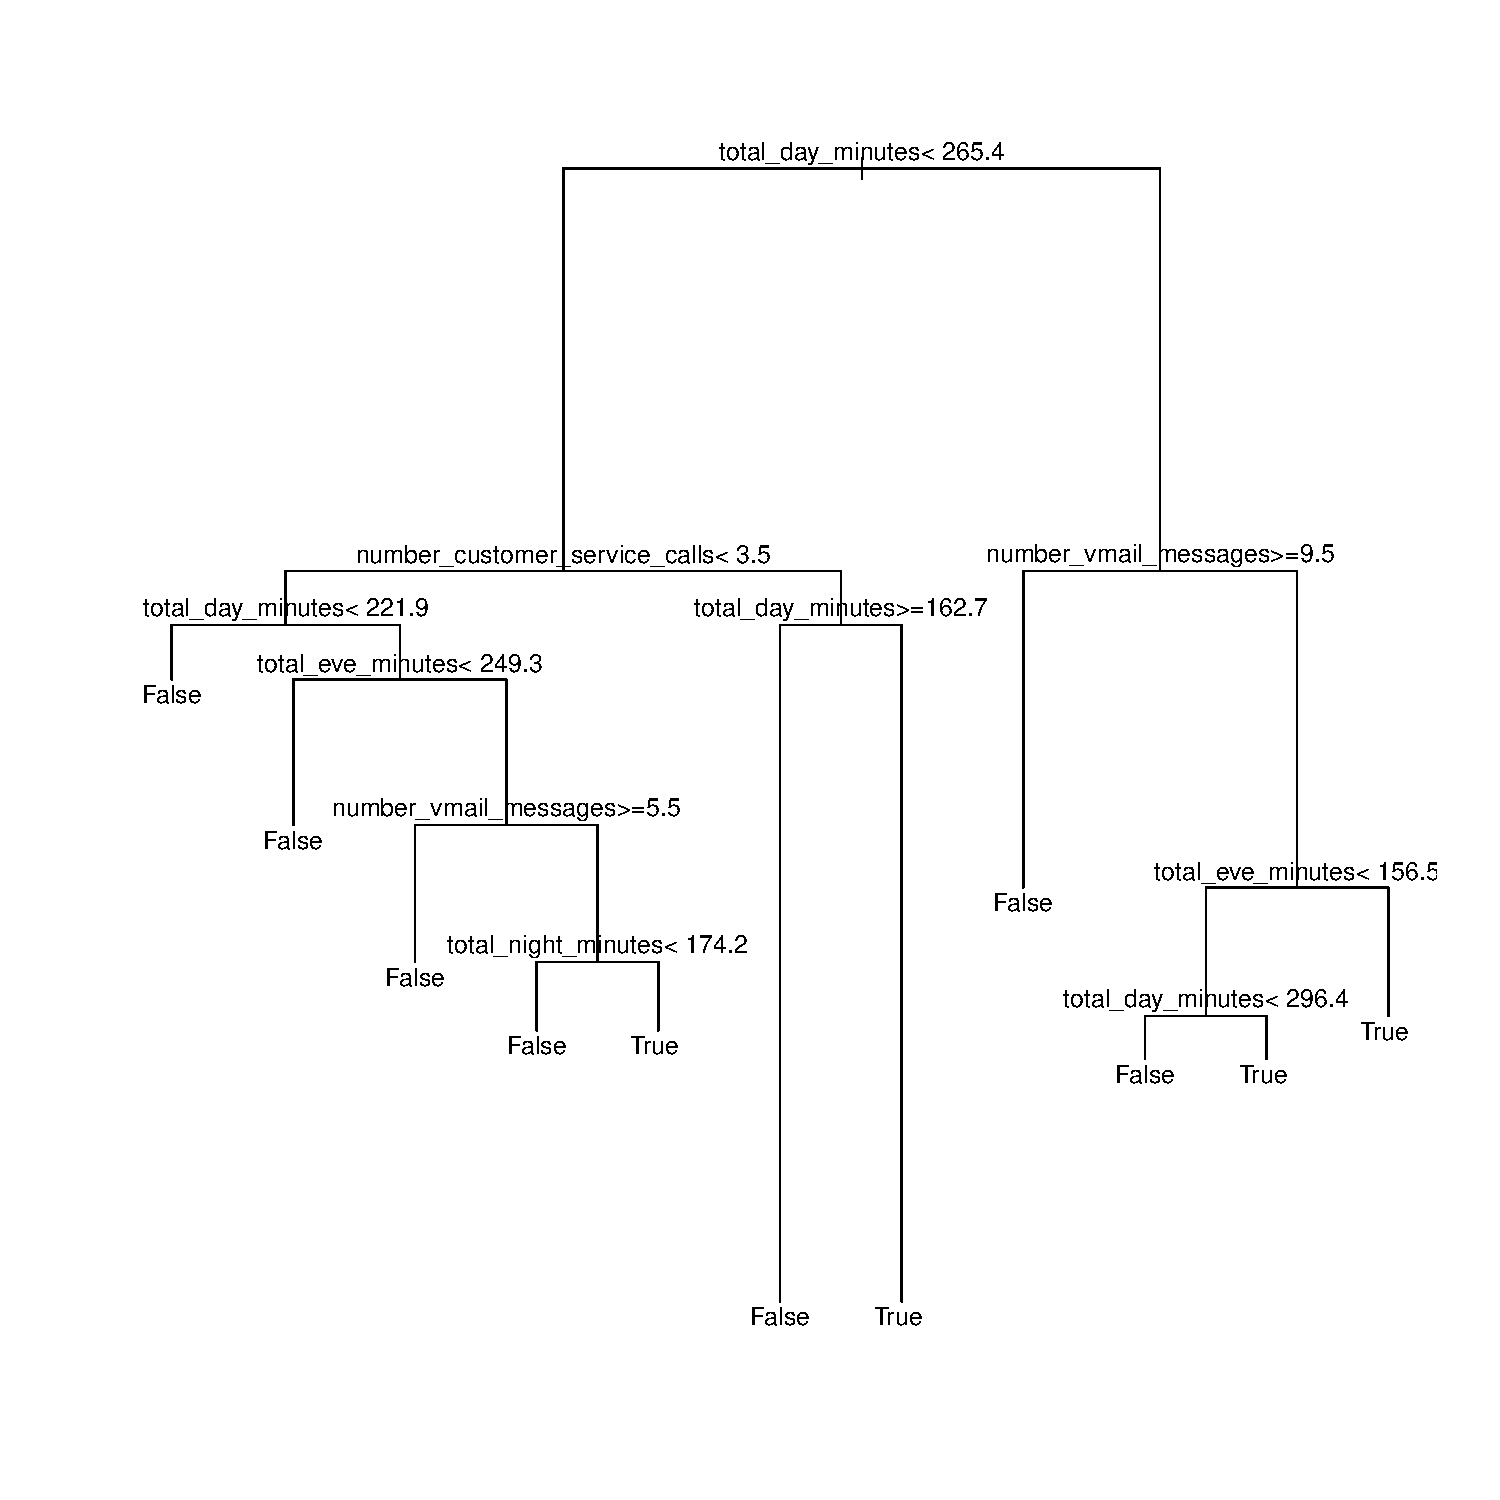
\includegraphics[width=18cm,height=20cm]{progress_presentaion/ppt_figures/churnDecisionTree}
		\end{figure}

\newpage
\subsection{Support vector machine}
I have trained and tested two SVM's linear kernel SVM and Radial kernel. The following are the statistics from the training of the SVM's
SVM linear kernel stats :
	\begin{itemize}
		\item Training sameple : 	3500
		\item Testing sample : 1500
		\item 18 predictors
		\item 2 classes: 'False', 'True' 
		\item Pre-processing: centered (69), scaled (69) 
		\item Resampling: Cross-Validated (10 fold, repeated 3 times) 
		\item Resampling results
		\begin{itemize}
			\item Accuracy  0.8595245
			\item Kappa      0.003825618 
		\end{itemize}
	\end{itemize}
	
	Confusion matrix linear kernel~\ref{svm-l-cm}
		\begin{table}[H]
							\centering
							\caption{SVM Linear confusion matrix}
							\label{svm-l-cm}
			\begin{tabular}{lll}
				\hline
				Prediction & False & True \\
				\hline
				False & 1285 & 215 \\
				\hline
				True & 0 & 0 \\
				\hline
			\end{tabular}
		\end{table}
			\begin{table}[H]
				\centering
				\caption{SVM Linear Stats}
				\label{svm-l-stats}
				\begin{tabular}{p{5cm}p{1cm}p{5cm}}
					Accuracy  & : & 0.8567 \\
					\hline
					95\% CI   & : & (0.8379, 0.874) \\ \hline
					No Information Rate  & : & 0.8567 \\ \hline
					P-Value {[}Acc \textgreater NIR{]}  & : & 0.5182 \\ \hline
					Sensitivity  & : & 1 \\ \hline
					Specificity  & : & 0 \\ \hline
					
				\end{tabular}
			\end{table}
			
			SVM radial kernel statistics
				\begin{itemize}
					\item Training sameple : 	3500
					\item Testing sample : 1500
					\item 18 predictors
					\item 2 classes: 'False', 'True' 
					\item Pre-processing: centered (69), scaled (69) 
					\item Resampling: Cross-Validated (10 fold, repeated 3 times) 
					%		\item Summary of sample sizes: 3150, 3151, 3150, 3150, 3150, 3149, ... 
					\item Resampling results
					\begin{itemize}
						\item Accuracy  0.8594297
						\item Kappa      0
					\end{itemize}
				\end{itemize}
				
				SVM radial kernel confusion matrix~\ref{svm-r-cm}
					\begin{table}[H]
						\centering
						\caption{SVM Radial confusion matrix}
						\label{svm-r-cm}
						\begin{tabular}{lll}
							\hline
							Prediction & False & True \\
							\hline
							False & 1266 & 68 \\
							\hline
							True & 19 & 147 \\
							\hline
						\end{tabular}
						
					\end{table}
						\begin{table}[H]
							\centering
							\caption{SVM Radial Stats}
							\label{svm-r-stats}
							\begin{tabular}{p{5cm}p{1cm}p{5cm}}
								Accuracy  & : & 0.8566667 \\
								\hline
								95\% CI   & : & (0.8379028, 0.8740215) \\ \hline
								No Information Rate  & : & 0.8566667  \\ \hline
								P-Value {[}Acc \textgreater NIR{]}  & : &  0.5181819 \\ \hline
								Sensitivity  & : & 1 \\ \hline
								Specificity  & : & 0 \\ \hline
								
							\end{tabular}
						\end{table}
			
\subsection{Neural networks}
To train the neural networks the churn data set needs to be transformed so that dimensions of data type factor are converted to numeric data type. This is my current 

\section{Dashboard of ICPCR}
The dashboard is prepared in shiny and below are a few screen-shots.

Figure~\ref{icpcr-1} enables the viewer to quickly scan the data set being used and understand the values of dimensions. A find search and sort functionality is also included.


		\begin{figure}[H]
			\caption{Dashboard 1}
			\label{icpcr-1}
			\hspace*{-3cm}
			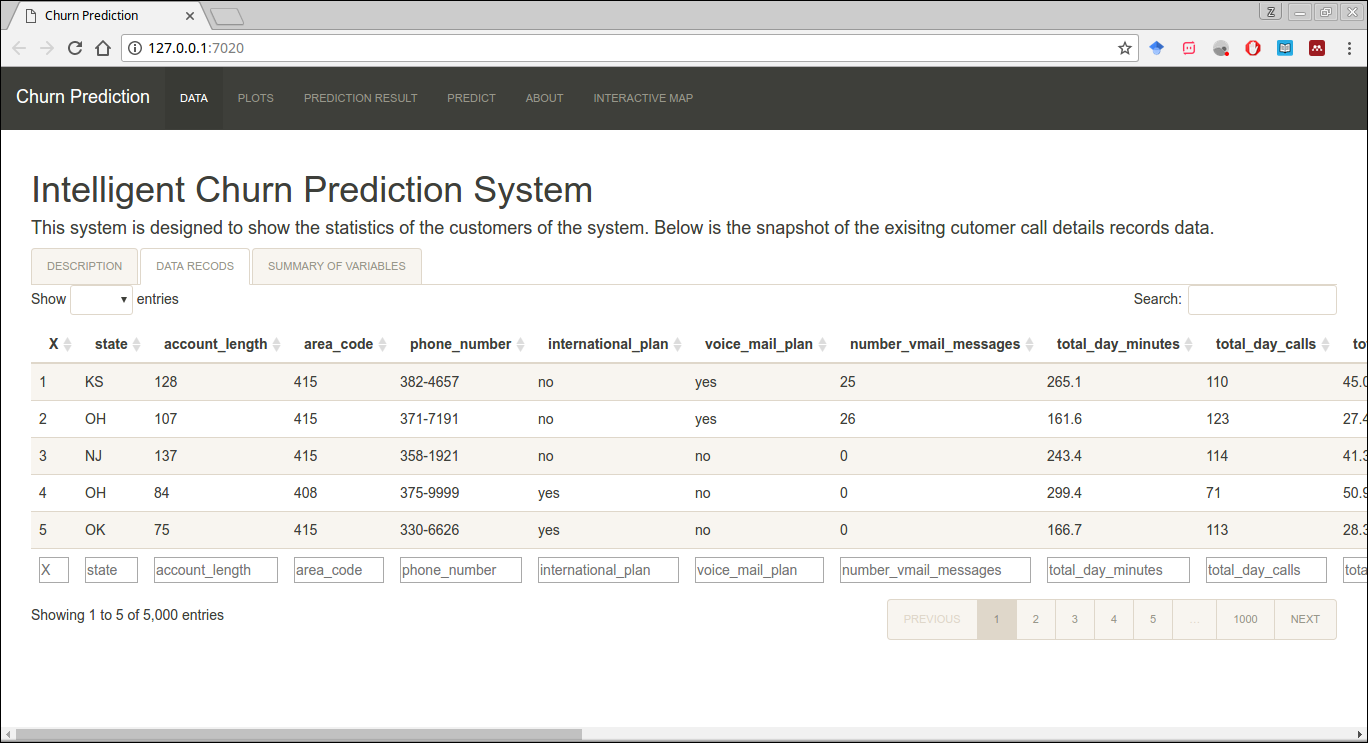
\includegraphics[scale=0.5]{progress_presentaion/ppt_figures/icpcr_1_dash.png}
		\end{figure}
		\newpage
Figure~\ref{icpcr-2} This describes the quantitative analysis of the dimensions.
		\begin{figure}[H]
			\caption{Dashboard 2}
			\label{icpcr-2}
			\hspace*{-2cm}
			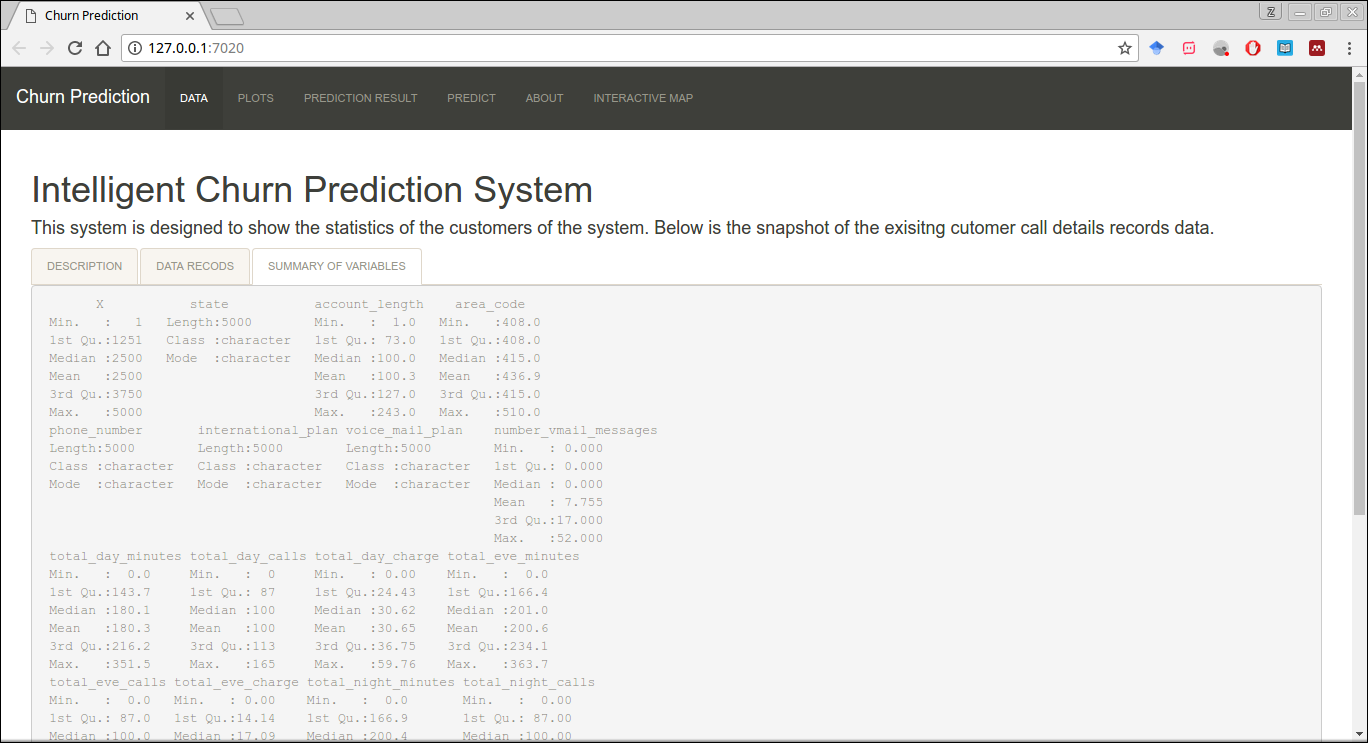
\includegraphics[scale=0.4]{progress_presentaion/ppt_figures/icpcr_2_dash.png}
		\end{figure}
		\newpage
Figure~\ref{icpcr-3} This displays the bar plot region wise for the churners to non-churners
		\begin{figure}[H]
			\caption{Dashboard 3}
			\label{icpcr-3}
			\hspace*{-2cm}
			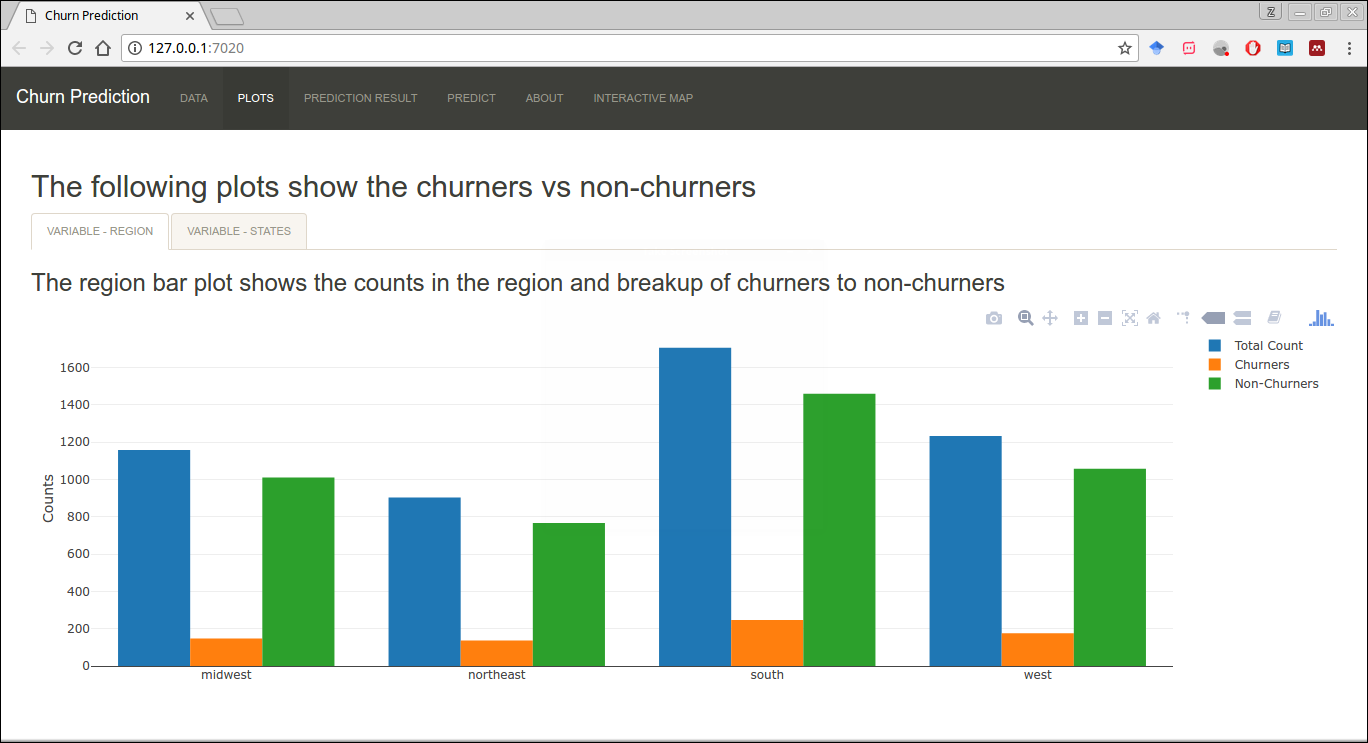
\includegraphics[scale=0.4]{progress_presentaion/ppt_figures/icpcr_3_dash.png}
		\end{figure}
		\newpage
Figure~\ref{icpcr-4} This displays the bar plot of the state wise churners to non-churners
		\begin{figure}[H]
			\caption{Dashboard 4}
			\label{icpcr-4}
			\hspace*{-2cm}
			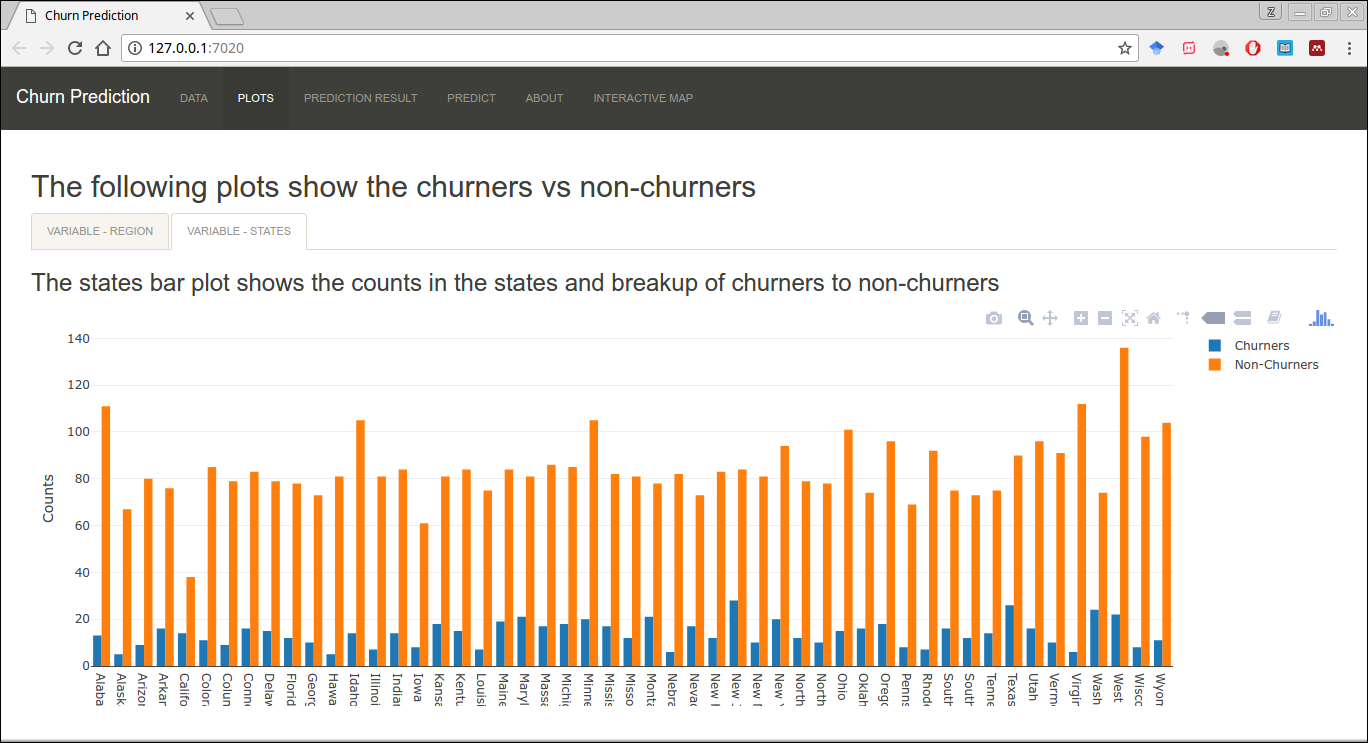
\includegraphics[scale=0.4]{progress_presentaion/ppt_figures/icpcr_4_dash.png}
		\end{figure}
		\newpage
Figure~\ref{icpcr-5} The screen shot is about a functionality to be implemented to enable the user to upload the data in CSV format to predict the churning of customers
		\begin{figure}[H]
			\caption{Dashboard 5}
			\label{icpcr-5}
			\hspace*{-2cm}
			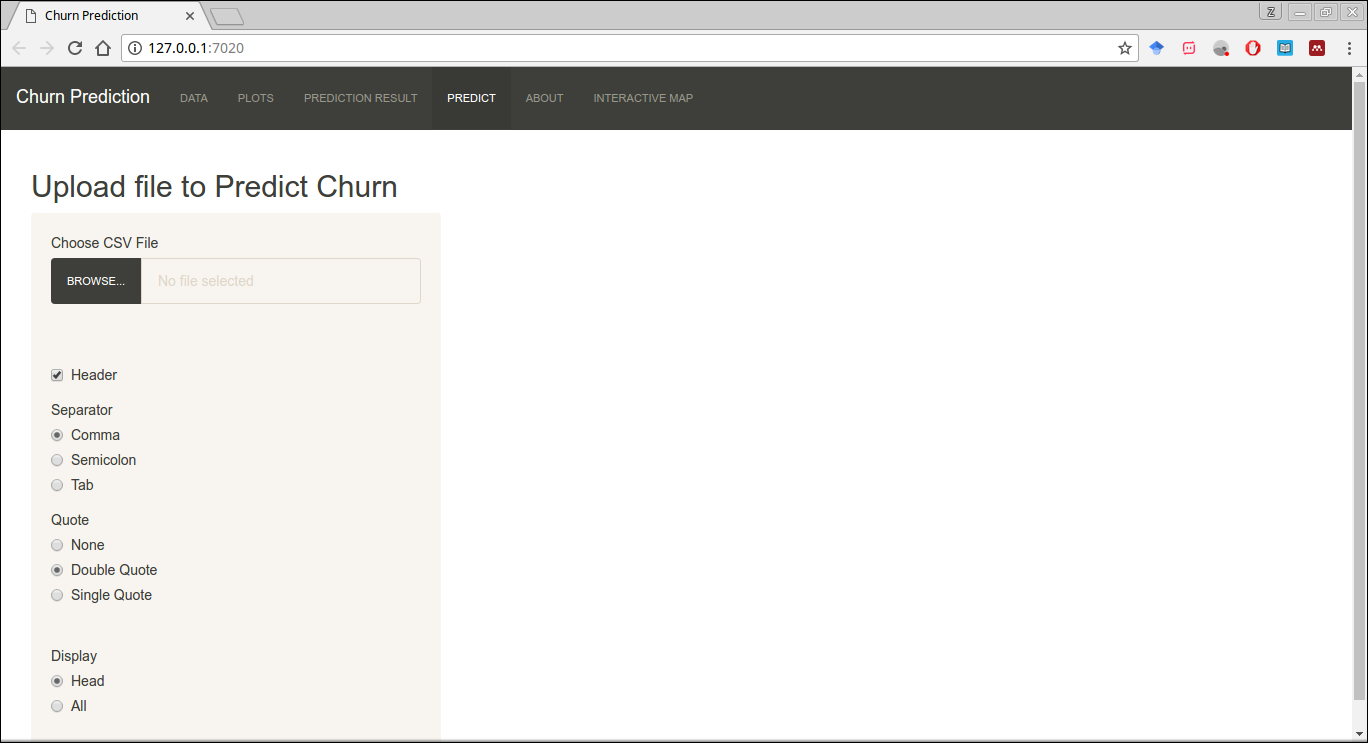
\includegraphics[scale=0.4]{progress_presentaion/ppt_figures/icpcr_5_dash.png}
		\end{figure}
		\newpage
Figure~\ref{icpcr-6} This functionality will be showing state wise distribution of telecom population and user will be able to customize to select churning or retaining populations.
		\begin{figure}[H]
			\caption{Dashboard 6}
			\label{icpcr-6}
			\hspace*{-2cm}
			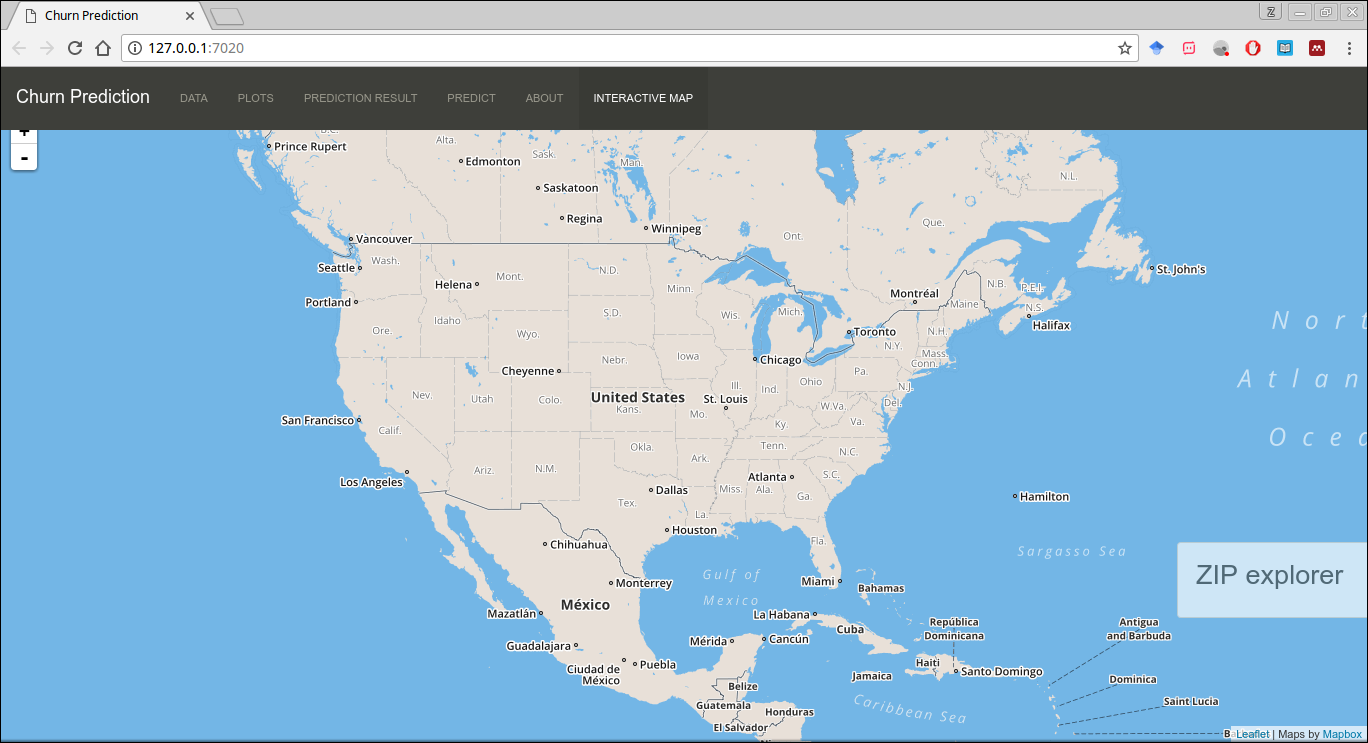
\includegraphics[scale=0.4]{progress_presentaion/ppt_figures/icpcr_6_dash.png}
		\end{figure}